\chapter{Background}\label{chap:background}

% what is structure/.... only technicall

% related work part vs background
%related work CNN
% more enter in details

%dataset in the method
%
% Background : explain the dataset, the pointer......
% assumption part on malloc header/pointer.....

% hardware in the ressources sections 

%make sure the code doesn't split

%key arent corrupted at least 2, at most 6

% 2-gram > bi-gram


\paragraph*{}Building upon our exploration of SSH key detection, we recognize that OpenSSH plays a pivotal role in secure communication. The heap dumps of OpenSSH, essentially memory snapshots, are rich reservoirs of data. By generating graphs from these dumps, intricate connections between data structures, identified via their malloc headers, and their corresponding pointers are revealed.

\paragraph*{}Our research delves into the intelligent embedding of connections derived from OpenSSH heap dumps. Beyond mere graph representations, it's essential to comprehend the raw byte sequences within these dumps. Traditional methods such as Shannon entropy, \acrfull{bfd}, and bigram frequencies form the foundation. However, the rise of deep learning has ushered in a range of sophisticated techniques. Models like \acrfull{rnn} \cite{lai_recurrent_2015} (including \acrfull{lstm}\cite{hochreiter_long_1997} and \acrfull{gru}\cite{chung_empirical_2014}), sequence-to-sequence learning \cite{sutskever_sequence_2014}, and convolutional approaches (\acrshort{cnn})\cite{lecun_gradient-based_1998} offer novel perspectives on raw byte embedding. The integration of \acrshort{cnn} with recurrent networks has proven effective in sequence modeling \cite{bai_empirical_2018}. Furthermore, neural networks, especially in lossless representations, have shown promise in file fragment classification \cite{hiester_file_2018}. Our exploration also encompasses the potential of transformers\cite{vaswani_attention_2017} and autoencoders.

\paragraph*{}To identify structures containing OpenSSH keys, we employ machine learning classifiers. Among the standard models, the Random Forest classifier stands out for its versatility and accuracy. Balancing strategies are crucial, especially when dealing with imbalanced datasets, to ensure that the classifier doesn't exhibit bias towards the majority class. In addition to classification, our research emphasizes clusterization techniques to group similar data points and ensure coherence. Algorithms such as DBSCAN and OPTICS are at the forefront of our clusterization approach, providing insights into the inherent groupings within the OpenSSH heap dump data.
\paragraph*{}The aim of this background section is to provide a comprehensive overview of graph creation from heap dumps, techniques for raw byte embedding, and their role in identifying OpenSSH key structures. By merging age-old techniques with modern approaches, we strive to highlight the most effective methods for analyzing OpenSSH heap dump.
        
\section{Traditional Statistical Embedding}\label{seq:background:traditional_statistical_embedding}

    \paragraph{}Within the domain of machine learning, how data is represented significantly impacts the performance of models. Even though traditional statistical embedding techniques have been around before many contemporary methods, they continue to be vital in readying data for machine learning endeavors. Rooted in statistical foundations, these techniques provide a methodical approach to transform raw data into concise and meaningful forms. In this subsection, we'll delve into the nuances of entropy and its role in byte sequence embedding, \acrfull{bfd}, and also highlight other classical statistical embedding methods pivotal in data representation for machine learning.
        
    \subsection{Entropy and its application in byte sequence embedding}
        \paragraph{}Entropy, a fundamental concept in information theory, quantifies the amount of uncertainty or randomness associated with a set of data. Introduced by Claude Shannon in his groundbreaking work \cite{shannon_mathematical_1948}, entropy serves as a measure of the average information content one can expect to gain from observing a random variable's value.

        \paragraph{}Mathematically, the entropy \(H(X)\) of a discrete random variable \(X\) with possible values \newline \(\{x_1, x_2, \ldots, x_n\}\) and probability mass function \(P(X)\) is given by:
        \begin{align}
            H(X) &= -\sum_{i=1}^{n} P(x_i) \log_2 P(x_i)
            \label{eq:shannon_entropy}
        \end{align}

        \paragraph{}Within the scope of identifying SSH keys, the significance of entropy cannot be understated. Byte sequences exhibiting high entropy typically reflect a multifaceted and varied informational content, traits that are synonymous with encryption keys, especially those in SSH. Sequences with pronounced entropy are often prime contenders for SSH keys due to their inherent randomness and lack of predictability, mirroring the attributes of robust security keys.

        \paragraph{}Fundamentally, entropy acts as a quantitative tool to evaluate the depth of information within data. When applied to SSH, it suggests that data sequences with elevated entropy levels have a heightened probability of correlating with secure keys. This positions entropy as an essential instrument for pinpointing and authenticating SSH keys.
    \subsection{Byte Frequency Distribution (BFD)}\label{seq:background:byte_frequency_distribution}
        \paragraph{}In the complex world of raw byte embedding, \acrfull{bfd} and n-gram embedding stand out as essential methods, each bringing unique benefits to data representation. \acrshort{bfd} zeroes in on the distribution of individual byte values in a raw byte sequence. Analyzing these distributions allows for the identification of patterns that reflect the inherent nature of the data. This embedding technique becomes particularly relevant when assessing the randomness or structure of byte sequences, such as when detecting encrypted data or pinpointing specific file signatures.

        \paragraph{}On the other hand, n-gram embedding dives deeper into raw byte sequences. Instead of focusing solely on individual bytes, it captures patterns formed by sequences of 'n' consecutive bytes. This approach garners a wider range of contextual information from the raw byte data. For example, a trigram (3-gram) examines patterns formed by three sequential bytes, providing a richer representation than single byte values. Yet, a challenge with n-gram embedding is the potential for the output vector size to grow exponentially as 'n' increases, posing computational and storage issues, especially in real-time scenarios.
        
        \paragraph{}In the realm of raw byte embedding, both \acrshort{bfd} and n-gram techniques offer invaluable perspectives. While \acrshort{bfd} establishes a base representation centered on individual byte frequencies, n-gram embedding enhances it by spotlighting the complex relationships and patterns among consecutive bytes. Together, they form a robust arsenal for representing and analyzing raw byte data in a variety of applications.
    \subsection{Other traditional statistical embedding techniques}
        \paragraph{Mean Byte Value}The Mean Byte Value represents the average value of all bytes in a given sequence. It provides an insight into the central tendency of the byte values in the sequence. Mathematically, for a byte sequence \( B \) of length \( n \):
        \begin{equation}
        \text{Mean Byte Value} = \frac{1}{n} \sum_{i=1}^{n} B_i
        \label{eq:mean_byte_value}
        \end{equation}

        \paragraph{Mean Absolute Deviation (MAD)}MAD measures the average distance of each byte value from the mean, providing a sense of the dispersion or spread of the byte values around the mean. It is given by:
        \begin{equation}
        \text{MAD} = \frac{1}{n} \sum_{i=1}^{n} |B_i - \text{Mean Byte Value}|
        \label{eq:mad}
        \end{equation}

        \paragraph{Standard Deviation}Standard Deviation quantifies the amount of variation or dispersion in the byte sequence. A higher value indicates greater variability in the byte values. It is defined as:
        \begin{equation}
        \text{Standard Deviation} = \sqrt{\frac{1}{n} \sum_{i=1}^{n} (B_i - \text{Mean Byte Value})^2}
        \label{eq:standard_deviation}
        \end{equation}

        \paragraph{Skewness}Skewness\cite{wheeler_problems_2011} measures the asymmetry of the distribution of byte values around the mean. A positive value indicates a distribution that is skewed to the right, while a negative value indicates a distribution skewed to the left. It provides insights into the shape of the distribution of byte values. The Fisher’s skewness\cite{cain_univariate_2017} is :
        \begin{equation}
        \text{Skewness} = \frac{n}{(n-1)(n-2)} \sum_{i=1}^{n} \left( \frac{B_i - \text{Mean Byte Value}}{\text{Standard Deviation}} \right)^3
        \label{eq:skewness}
        \end{equation}

        \paragraph{Kurtosis}Kurtosis\cite{wheeler_problems_2011} measures the "tailedness" of the distribution of byte values. A higher kurtosis value indicates a distribution with heavier tails, while a lower value indicates lighter tails. It provides insights into the extremities of the distribution. The Fisher’s kurtosis\cite{cain_univariate_2017} is :
        \begin{equation}
        \text{Kurtosis} = \frac{n(n+1)}{(n-1)(n-2)(n-3)} \sum_{i=1}^{n} \left( \frac{B_i - \text{Mean Byte Value}}{\text{Standard Deviation}} \right)^4 - \frac{3(n-1)^2}{(n-2)(n-3)}
        \label{eq:kurtosis}
        \end{equation}

        \paragraph{n-gram on Bits}When applying n-gram techniques to bits instead of bytes, we focus on sequences of 'n' consecutive bits. For example, a 2-gram on bits would consider patterns formed by two consecutive bits, resulting in four possible combinations: 00, 01, 10, and 11. This approach significantly reduces the size of the output vector compared to byte-based n-grams. By focusing on bits, we can capture more granular patterns in the data while benefiting from a more compact representation, which is computationally efficient and requires less storage.

\section{Deep Learning Models for Raw Byte Embedding}\label{seq:background:deep_learning_models_for_raw_byte_embedding}

    \paragraph{}In the area of data representation, deep learning is great for understanding raw byte sequences. Just like these models are good at understanding text, they're also good at understanding raw bytes. They can learn and show sequences on their own, which is really helpful for both text and raw bytes. In this section, we'll look at different deep learning models and how they work with raw byte embedding.

    \paragraph{}We'll start with \acrfull{rnn}. Just like they're good with word sequences in text, \acrfull{rnn} are also good with raw byte sequences. Then, we'll look at \acrfull{cnn}, which can find patterns in raw bytes, just like they find patterns in text. After that, we'll talk about Autoencoders, which can learn in a special way. To finish this section, we'll discuss Transformers. They're good at understanding data over a long time, similar to how they understand text.

    \subsection{RNNs : Understanding sequence data}
        \paragraph{}\acrfull{rnn} are great tools for text classification. They're good at understanding the deeper meanings in text. Unlike older models that use hand-made features, \acrshort{rnn} can learn and show sequences on their own. This makes them really useful for tasks that deal with sequences. When we think about embedding raw bytes, \acrshort{rnn}'s skill in understanding sequences is similar to how they handle word sequences in text. Here is a list of different \acrshort{rnn} models and their advantages and disadvantages.

        \paragraph{\acrfull{rcnn} for Text Classification\cite{lai_recurrent_2015}:} The \acrshort{rcnn} model, as discussed in the paper by Lai et al., is designed specifically for text classification. Unlike traditional models, \acrshort{rcnn} do not rely on handcrafted features. Instead, they employ a recurrent structure to capture contextual information about words. This approach is believed to introduce considerably less noise compared to traditional window-based neural networks. The model's bidirectional structure ensures that both preceding and succeeding contexts of a word are considered, enhancing its understanding of the word's semantics.

        \begin{itemize}
            \item \textbf{Advantages:} 
            \begin{itemize}
                \item No need for handcrafted features.
                \item Captures richer contextual information.
                \item less noisy.
            \end{itemize}
            \item \textbf{Disadvantages:} 
            \begin{itemize}
                \item Complexity due to bidirectional structure.
                \item Might require more computational resources.
            \end{itemize}; 
        \end{itemize}

        \paragraph{\acrfull{lstm}\cite{hochreiter_long_1997}:}The \acrshort{lstm}, introduced by Hochreiter and Schmidhuber, is a specialized form of \acrshort{rnn} designed to combat the vanishing gradient problem inherent in traditional \acrshort{rnn}. The vanishing gradient problem arises when gradients of the loss function, which are used to update the network's weights, become too small for effective learning. This typically happens in deep networks or when processing long sequences, causing the earlier layers or time steps to receive minimal updates. As a result, traditional \acrshort{rnn} struggle to learn long-term dependencies in the data.

        \paragraph{}\acrshort{lstm} address this issue with their unique cell state and gating mechanisms. The cell state acts as a "conveyor belt" that can carry information across long sequences with minimal changes, ensuring that long-term dependencies are captured. The gating mechanisms, namely the input, forget, and output gates, regulate the flow of information into, out of, and within the cell. This design allows LSTMs to selectively remember or forget information, making them adept at learning and retaining long-term dependencies in sequences.

        \begin{itemize}
            \item \textbf{Advantages:}
            \begin{itemize}
                \item Efficiently learns long-term dependencies; overcomes the vanishing gradient problem inherent in traditional \acrshort{rnn}.
                \item Often achieves faster and more stable learning.
            \end{itemize}
            \item \textbf{Disadvantages:}
            \begin{itemize}
                \item More complex architecture compared to basic \acrshort{rnn} and even \acrshort{gru}.
                \item Can be computationally intensive due to the multiple gating mechanisms.
            \end{itemize}
        \end{itemize}

        \paragraph{\acrfull{gru}\cite{chung_empirical_2014}:} \acrshort{gru} are a variant of \acrshort{rnn} that aim to capture long-term dependencies without the complexity of \acrshort{lstm}. They use a gating mechanism to control the flow of information, making them efficient in sequence modeling tasks.

        \begin{itemize}
            \item \textbf{Advantages:} 
            \begin{itemize}
                \item Simplified structure compared to \acrshort{lstm}.
                \item Efficient in capturing long-term dependencies.
                \item Sometimes outperforms \acrshort{lstm}.
            \end{itemize}
            \item \textbf{Disadvantages:} 
            \begin{itemize}
                \item Still more complex than traditional \acrshort{rnn}.
                \item Might not always outperform \acrshort{lstm} in all tasks.
            \end{itemize}
        \end{itemize}
        

        \paragraph{}To sum it up, \acrshort{rnn} are good at understanding sequences and context. This makes them a good choice for embedding raw bytes. Just like they understand words based on the words around them, \acrshort{rnn} can find patterns in raw byte sequences, giving us a better understanding of the data.
    \subsection{CNNs : Pattern detection in raw bytes}
        \paragraph{}\acrfull{cnn}\cite{lecun_gradient-based_1998} are a specialized category of deep learning models adept at identifying patterns. Originally designed for visual data, their prowess extends to tasks like image and document recognition. Drawing inspiration from the human visual cortex's biological processes, \acrshort{cnn} are architected to autonomously and adaptively discern spatial feature hierarchies from inputs. This becomes particularly relevant when considering raw byte embedding, where the goal is to detect patterns in sequences of bytes. The CNN architecture boasts convolutional layers that perform operations on input data to capture localized patterns, and pooling layers that condense spatial dimensions while preserving crucial information. This layered approach enables \acrshort{cnn} to detect intricate patterns by progressively building on simpler foundational patterns. When applied to byte sequences or document recognition, \acrshort{cnn} excel, showcasing remarkable efficacy, especially in tasks like identifying patterns within raw byte sequences or recognizing handwritten content.

        \paragraph{}When tailored to \acrshort{cnn}, the \acrfull{seq2seq}\cite{gehring_convolutional_2017} approach emerges as a potent tool for transforming raw byte sequences into meaningful embeddings. The encoder segment of the \acrshort{seq2seq} model is central to this transformation. It delves into the byte sequence, discerning intricate patterns and nuances, and distills this rich information into a concise context vector or embedding. This condensed representation captures the core essence of the byte sequence, positioning it as a valuable input for subsequent tasks, such as classification models.

        \paragraph{}At the heart of the encoder lie the convolutional layers, skilled in pinpointing specific patterns within the byte sequence. Whether it's unique byte combinations or indicative n-grams, these layers are primed to detect them. As they traverse the raw byte sequence, they employ specialized filters, honed to recognize these specific patterns. As the data flows through the encoder's layers, these identified patterns are synthesized and refined, culminating in a comprehensive embedding of the sequence.

        \paragraph{}Here are two \acrfull{seq2seq} models using \acrshort{cnn} :
        

        \begin{itemize}
            \item \textbf{Autoencoders:} These neural network architectures\cite{hinton_reducing_2006} are designed for data compression and reconstruction. The encoder part compresses the input data into a compact representation, while the decoder reconstructs the original data from this representation. In the context of raw byte sequences, the encoder can be used to generate embeddings that capture the essential patterns and structures of the data.

            \item \textbf{Transformers :} Transformers\cite{vaswani_attention_2017} utilize self-attention mechanisms to weigh the significance of different parts of the input data. This allows them to capture long-range dependencies and relationships in the data. When applied to raw byte sequences, transformers can generate embeddings that consider both local and global patterns, making them particularly effective for tasks that require understanding the broader context of a sequence.

        \end{itemize}
        
        \paragraph{}Yet, a significant challenge with traditional \acrfull{seq2seq} models using \acrshort{cnn} is their constraint in managing inputs of varying sizes. Constructed with a set input size, they face difficulties when presented with sequences of diverse lengths, like raw byte sequences.

        \paragraph{}To address this limitation, various techniques have been employed to normalize the size of the input data. One of the most common methods is \textbf{padding}, where shorter sequences are filled with predefined placeholder values (often zeros) until they match the length of the longest sequence in the dataset. This ensures that all sequences fed into the model have a uniform length. Another approach is \textbf{bucketing}, where sequences of similar lengths are grouped together, minimizing the amount of padding required. Additionally, \textbf{truncation} can be used to shorten sequences that exceed a certain length, although this might result in the loss of some information. While these techniques enable \acrshort{cnn}-based \acrfull{seq2seq} models to handle variable-sized inputs, it's crucial to ensure that the preprocessing steps do not introduce noise or distort the inherent patterns and relationships within the raw byte sequences.
\section{Graph Embedding Methods}
    \paragraph{}Graph embedding techniques focus on the mapping of nodes and edges within a graph onto vectors within a lower-dimensional space \cite{hogan_knowledge_2022}. The primary objective is to retain the structural properties of the graph, such as node connectivity and community structure, in this embedded space. These resulting vectors find application in diverse machine learning tasks, including clustering, classification, and link prediction. For a comprehensive exploration of these techniques, "Knowledge Graphs" offers a detailed overview. Some noteworthy techniques in this domain encompass:

    \begin{enumerate}
        \item \textbf{Translational Models:} These graph embedding techniques revolve around translational models that interpret edge labels as transformations from subject nodes to object nodes \cite{hogan_knowledge_2022}.
        
        \begin{itemize}
            \item \textbf{TransE:} One of the earliest and straightforward translational models, TransE represents entities as points in a vector space and relations as translations between these points. The core idea is that for a valid triple (h, r, t), the equation $h+r = t$ should hold, with $h$ representing the head entity, $r$ denoting the relation, and $t$ standing for the tail entity. While simple and computationally efficient, this model has limitations in capturing complex relationships \cite{hogan_knowledge_2022}.
            
            \item \textbf{TransH:} Extending TransE, TransH introduces relation-specific hyperplanes. This extension allows the model to capture more intricate relationships by projecting entity embeddings onto these hyperplanes before performing translations \cite{hogan_knowledge_2022}.
            
            \item \textbf{TransR:} Going a step further than TransH, TransR not only introduces relation-specific hyperplanes but also relation-specific translations. This flexibility enables a more versatile representation of relations, accommodating various complexities \cite{hogan_knowledge_2022}.
            
            \item \textbf{Other Developments:} Noteworthy advancements include TransD and MuRP, highlighting the active research in this domain \cite{hogan_knowledge_2022}.
        \end{itemize}

        \item \textbf{Tensor Decomposition Models} These models represent entities and relations as vectors or matrices within a lower-dimensional space, grounded in the assumption that the relationship between entities can be expressed through a bilinear function. While they are computationally efficient and capable of capturing complex relationships, they do have limitations in modeling asymmetric and reflexive relations.

        \begin{itemize}
            \item \textbf{RESCAL:} RESCAL employs a bilinear model, where each relation is represented by a full-rank matrix. This approach allows for the representation of asymmetric and reflexive relations but comes at the cost of increased computational complexity \cite{hogan_knowledge_2022}.
            
            \item \textbf{DistMult:} DistMult simplifies RESCAL by assuming that the relation matrices are diagonal. This simplification reduces the number of parameters and computational complexity, making it a more scalable option \cite{hogan_knowledge_2022}.
            
            \item \textbf{ComplEx:} ComplEx extends DistMult by introducing complex-valued embeddings. This addition enables the model to effectively capture asymmetric relations while maintaining computational efficiency \cite{hogan_knowledge_2022}.
        \end{itemize}

        \item \textbf{Neural Models} Neural models leverage neural networks to acquire the features of entities and relations, offering a flexible and adaptive approach to graph embeddings.

        \begin{itemize}
            \item \textbf{ConvKB:} ConvKB employs a convolutional neural network to autonomously learn entity and relation features. While technically a translational model, it uses a convolutional layer to capture interactions between entities and relations, providing a flexible and adaptable approach to graph embeddings \cite{nguyen_novel_2018}.
            
            \item \textbf{RotatE:} RotatE introduces complex rotations in the embedding space to model relations. This neural model offers a more expressive approach to capturing relation semantics \cite{hogan_knowledge_2022}.
            
            \item \textbf{SDNE (Structural Deep Network Embedding):} SDNE uses a deep autoencoder to acquire complex and non-linear node embeddings while preserving first-order and second-order proximities. It is particularly effective in capturing intricate patterns and structures within the graph \cite{wang_structural_2016}.
            
            \item \textbf{R-GCN (Relational Graph Convolutional Networks):} R-GCNs combine the strengths of Graph Convolutional Networks (GCNs) and traditional embedding methods, capturing both topological and semantic information \cite{schlichtkrull_modeling_2018}. A recent study by Degraeve et al. highlights the importance of the message passing paradigm in R-GCN and introduces a variant called Random R-GCN (RR-GCN) \cite{degraeve_r-gcn_2022}.
            
            \item \textbf{ConvE:} ConvE employs convolutional layers to capture local and global interactions between entities and relations, offering a more expressive representation \cite{hogan_knowledge_2022}.
        \end{itemize}

        \item \textbf{Language Models}
        Language models harness pre-trained language models to enrich embeddings with contextual information, tapping into recent advancements in language modeling to grasp the semantics of entities and relations.

        \begin{itemize}
            \item \textbf{BERT for KGE (Knowledge Graph Embedding):} This approach utilizes pre-trained BERT models, capitalizing on the capabilities of language models to enhance embeddings with contextual information \cite{yao_kg-bert_2019}.
            
            \item \textbf{BART KGE:} Bidirectional and Auto-Regressive Transformers (BART) serve as denoising autoencoders suitable for various NLP tasks. This method employs BART to acquire entity and relation embeddings, and the associated paper also compares it with other Large Language Models (LLMs) like GPT-2 \cite{liu_kg-bart_2021}.
            
            \item \textbf{It's worth noting that the field of NLP is continuously evolving, with ongoing developments and emerging approaches.}
        \end{itemize}
    \end{enumerate}


\section{Machine learning}\label{seq:background:machine_learning}
    \paragraph{}Machine learning, an integral part of artificial intelligence, revolves around designing algorithms and statistical models that allow computers to perform tasks without being directly programmed. Instead of relying on detailed instructions for every task, machine learning techniques empower systems to learn from data and make data-driven decisions. A key method in this field is supervised learning, in which models are trained using data that comes with predefined labels. Here, each piece of data in the training set has an associated known output. The primary goal of supervised learning is to establish a relationship between inputs and outputs, enabling the model to predict or categorize new, unseen data based on this relationship.

    \paragraph{}A cornerstone in this realm is feature engineering, which involves the meticulous process of selecting and transforming variables to optimize model performance. Another challenge frequently encountered by practitioners is dealing with datasets where some classes are overrepresented, which can skew model predictions. Among the myriad of machine learning models available, certain ones have gained prominence due to their versatility and effectiveness. We will provide an overview of some of these notable models.

    \subsection{Features engineering}
        \paragraph{}Feature engineering\cite{khurana_feature_2017} is a cornerstone in the realm of machine learning. It involves the artful transformation of the given feature space to optimize the performance of predictive models. The significance of feature engineering cannot be overstated; it serves as a bridge between raw data and the predictive models, ensuring that the models are fed with the most relevant and informative features. Properly engineered features can drastically reduce modeling errors, leading to more accurate and reliable predictions. Here are some of the most common feature engineering techniques:

        \begin{itemize}
            \item \textbf{Normalization and Scaling }are preprocessing techniques used to standardize the range of independent features in the data. Many machine learning algorithms, especially those that rely on distance calculations like k-means clustering or support vector machines, are sensitive to the scale of the data. If features are on different scales, one feature might dominate others, leading to suboptimal model performance. Normalization typically scales features so that they have a unit norm, while other scaling methods, such as Min-Max scaling, transform features to lie in a given range, usually [0,1]. Z-score normalization or standard scaling is another method where features are scaled based on their mean and standard deviation. Properly scaled data ensures that each feature contributes equally to the model's decision, leading to more stable and accurate predictions.

            \item \textbf{Interaction Features\cite{khalid_survey_2014} }refer to the creation of new features by combining two or more existing features, aiming to capture any synergistic effect between them. In many cases, the interaction between variables can provide more information than the individual variables themselves. For instance, while analyzing real estate prices, the individual features 'number of rooms' and 'location' might be informative, but their interaction, 'number of rooms in a specific location', might offer even more predictive power. Interaction features can be created by multiplying, adding, or even dividing original features, and they can help in capturing non-linear relationships in the data, enhancing the model's ability to make accurate predictions.

            \item \textbf{Feature Selection\cite{khalid_survey_2014} }is a critical process in the machine learning pipeline that focuses on selecting the most relevant features from the original set, aiming to reduce the dimensionality and improve model performance. The primary goal is to eliminate redundant or irrelevant features that don't contribute significantly to the predictive power of the model. This not only helps in reducing the computational cost but also can lead to a more interpretable model. There are various techniques for feature selection, including filter methods (based on statistical measures), wrapper methods (like recursive feature elimination), and embedded methods (where algorithms inherently perform feature selection, such as decision trees). By judiciously selecting features, one can build efficient models that are less prone to overfitting and have better generalization capabilities.
        \end{itemize}

        \subsubsection{Correlation tests}\label{seq:background:correlation_tests}
            \paragraph{}To assess feature quality, various statistical measures come into play, including correlation tests that gauge the strength and direction of relationships between variables. Pearson, Kendall, and Spearman correlation coefficients are frequently employed to quantify linear or monotonic associations between each feature and the target variable \cite{boddy_statistical_2009}. A high absolute value of these coefficients indicates a robust relationship, aiding in feature selection.

            \begin{itemize}
                \item \textbf{Pearson Correlation:} This measures linear relationships between two variables, ranging from -1 to 1. -1 signifies a strong negative linear correlation, 1 suggests a strong positive linear correlation, and 0 implies no linear correlation.

                \item \textbf{Kendall’s Tau:} This non-parametric test gauges the strength and direction of a monotonic relationship between two variables.

                \item \textbf{Spearman’s Rank:} Also non-parametric, it assesses how well an arbitrary monotonic function can describe the relationship between two variables without making assumptions about frequency distribution.
            \end{itemize}
        
            \paragraph{}These techniques are valuable for evaluating relationships between each feature and generating correlation matrices, which, in turn, help identify redundant features. Univariate feature selection techniques allow the evaluation of each feature independently. In Python's scikit-learn library \cite{pedregosa_scikit-learn_2011}, methods like the F-test value and p-value are often used for this purpose.

            \begin{itemize}
                \item \textbf{F-test value:} This measures the linear dependency between the feature variable and the target. A higher F-test value suggests a more useful feature.

                \item \textbf{p-value:} It indicates the probability of an F-test value as large as observed arising if the null hypothesis is true. A smaller p-value implies rejecting the null hypothesis, indicating the feature's significance.
            \end{itemize}
            \paragraph{}In summary, features constitute the foundational elements of any machine learning model. The quality of these features, their processing, and utilization significantly impact the model's performance. Feature engineering is of paramount importance, as properly engineered features can substantially reduce modeling errors, leading to more accurate and reliable predictions. It serves as a crucial link between raw data and predictive models, ensuring that models are fed with the most relevant and informative features.

        \subsubsection{Dimensionnality reduction}

            \paragraph{}Following the aforementioned techniques, another essential facet in the feature engineering landscape is dimensionality reduction. As data grows in complexity, it often encompasses a vast number of features, leading to what is known as a high-dimensional space. While a plethora of features might seem advantageous, it introduces challenges, notably the \textit{curse of dimensionality}\cite{hutchison_curse_2005, koppen_curse_2000}. In such high-dimensional realms, data points tend to become increasingly sparse. This sparsity means that the relative distances between data points start to appear uniform, making it arduous for algorithms to discern meaningful patterns. This can lead to models that overfit the training data, capturing noise rather than the underlying data distribution. Additionally, the computational overhead increases, and deriving intuitive insights from the data becomes a daunting task.

            \paragraph{}Dimensionality reduction techniques come to the rescue by striving to trim down the number of features while preserving the crux of the information. Techniques like \acrfull{pca} and \acrfull{t-sne} are employed to transform the data from its original high-dimensional space to a more manageable, lower-dimensional one. This transformation aims to retain the significant patterns and structures inherent in the data. By judiciously reducing the dimensionality, not only can models be trained more efficiently, but they often yield better performance by focusing on the most pertinent features. This streamlined approach mitigates the challenges posed by the curse of dimensionality, ensuring models that are both robust and interpretable.

    \subsection{Imbalanced data}\label{seq:background:imbalanced_data}
        \paragraph{}In machine learning, a frequent obstacle is the presence of datasets where one category vastly overshadows others\cite{ramyachitra_imbalanced_2014}. This imbalance can skew models towards predicting the dominant class, often neglecting the less prevalent but potentially more critical class.

        \paragraph{}To counteract this, a variety of techniques have been devised:
        \begin{itemize}
            \item \textbf{Resampling:} This encompasses both increasing instances of the minority class (oversampling) and decreasing instances of the majority class (undersampling). A notable method for oversampling is the \acrfull{smote}, which generates artificial data points in the feature space.
            \item \textbf{Weighted Loss:} This strategy involves assigning greater weights to the minority class during the training phase, ensuring the model gives it due consideration.
            \item \textbf{Ensemble Methods:} Approaches such as bagging and boosting can be tailored to ensure a balanced class representation. For example, in bagging, each sample can be structured to maintain a balanced class ratio.
            \item \textbf{Anomaly Detection:} This method reframes the task from classification to anomaly detection, viewing the minority class as an outlier or anomaly.
        \end{itemize}
        \paragraph{}Selecting an appropriate strategy hinges on the specific problem and dataset characteristics. It's also crucial to evaluate the model's efficacy using suitable metrics, ensuring it genuinely addresses the imbalance.

    \subsection{Some common models}\label{seq:background:some_ml_common_models}
    \begin{itemize}
        \item \textbf{Logistic Regression\cite{nick_logistic_2007} : }Logistic regression serves as a statistical technique tailored for binary classification tasks. While linear regression is designed to forecast continuous outcomes, logistic regression focuses on predicting the likelihood of a binary result. It leverages the logistic function to relate multiple independent variables to a binary outcome, ensuring the predicted values fall between 0 and 1. Typically, a 0.5 threshold is used to classify the final outcome. A key strength of logistic regression is its clarity and ease of interpretation, though it might face challenges with complex non-linear data unless further feature adjustments are made.
        
        \item \textbf{Decision Trees\cite{kotsiantis_decision_2013} : }Decision trees are machine learning models designed for both classification and regression tasks. They segment data into subsets based on feature values, making decisions at each node. While their hierarchical structure offers easy visualization and interpretation, they can be prone to overfitting. However, strategies like pruning can help in refining the tree and mitigating overfitting.
        
        \item \textbf{Random Forest\cite{probst_hyperparameters_2019} : }Random Forest is an ensemble method that creates a 'forest' of decision trees. Each tree is trained on a random subset of the data and makes its own predictions. The Random Forest algorithm then aggregates these predictions to produce a final result. This method is known for its high accuracy, ability to handle large datasets with higher dimensionality, and its capacity to manage missing values.
        
        \item \textbf{\acrfull{svm}\cite{wu_analysis_2006} : }\acrshort{svm} are used for both regression and classification problems. They work by finding the hyperplane that best divides a dataset into classes. SVMs are effective in high-dimensional spaces and are versatile, as different Kernel functions can be specified for the decision function.
        
        \item \textbf{\acrfull{knn}\cite{laaksonen_classification_1996} :}\acrshort{knn} is a simple, instance-based learning algorithm. To make a prediction for a new data point, the algorithm finds the 'k' training examples that are closest to the point and returns the most common output value among them.
    \end{itemize}


    \subsection{Random Forest classifier model}\label{seq:background:random_forest}

        \paragraph{}Random Forest, as introduced earlier, is an ensemble learning method that operates by constructing multiple decision trees during training and outputting the mode of the classes for classification tasks or mean prediction for regression tasks. Let's delve deeper into its workings, advantages, and disadvantages.

        \subsubsection{How Random Forest Works}

        \begin{enumerate}
            \item \textbf{Bootstrap Aggregating (Bagging):} Random Forest begins by creating multiple datasets using bagging. It randomly selects samples from the original dataset with replacement, ensuring diversity in the datasets.
            
            \item \textbf{Constructing Decision Trees:} For each of these datasets, a decision tree is constructed. However, instead of using all features to make a decision at a node, a random subset of features is chosen. This introduces further randomness into the model and ensures that the trees are uncorrelated.
            
            \item \textbf{Aggregation:} Once all the trees are constructed, predictions are made by each tree. For classification, the mode of all the predictions is taken as the final prediction.
        \end{enumerate}

        \subsubsection{Advantages of Random Forest}

        \begin{itemize}
            \item \textbf{Accuracy:} Random Forests often produce highly accurate predictions as they combine the output of multiple decision trees.
            
            \item \textbf{Overfitting:} The model is less prone to overfitting due to the randomness introduced in its construction.
            
            \item \textbf{Handling Missing Data:} Random Forest can handle missing values by either using median values to replace continuous variables or computing the proximity-weighted average of missing values.
            
            \item \textbf{Feature Importance:} It provides insights into the importance of different features in making predictions.
        \end{itemize}

        \subsubsection{Disadvantages of Random Forest}

        \begin{itemize}
            \item \textbf{Complexity:} Random Forest creates a lot of trees (unlike only one tree in the case of decision tree) and combines their outputs. This makes the model more complex and computationally intensive.
            
            \item \textbf{Longer Training Time:} Due to the construction of multiple trees, the training time can be longer compared to other algorithms.
            
            \item \textbf{Less Intuitive:} While individual decision trees are simple and can be visualized, a forest is more challenging to interpret due to its ensemble nature.
        \end{itemize}

        \paragraph{}In conclusion, while Random Forest offers high accuracy and is robust against overfitting, it comes with increased complexity and training time. However, its advantages often outweigh the disadvantages, making it a popular choice for various machine learning tasks.

\section{Clustering}
    \paragraph{}Clustering is a key technique in unsupervised machine learning, aiming to group similar data points together. It's all about ensuring that items within a cluster are more alike than those in different clusters. This approach is great for uncovering hidden patterns in data. When it comes to checking the quality of an embedding, clustering can be a handy tool. By forming clusters from embedded data, we can see how effectively similar structures come together. A top-notch embedding should make sure that data points from the same structure cluster closely. So, by looking at how well clustering works, we can gauge the strength of the embedding.

    \subsection{K-Means Clustering}
        \paragraph*{}K-Means~\cite{macqueen_methods_1967} is a popular clustering method recognized for its straightforwardness and speed. It works by dividing a dataset into 'K' unique, separate groups (or clusters) based on how close each data point is to the cluster's center, termed the centroid. The method repeatedly places each data point with the closest centroid and then updates the centroid's position based on the points in its cluster. This cycle repeats until the centroids no longer move significantly. Though K-Means is great for clusters that are roughly spherical and similar in size, deciding on the best number of clusters (K) in advance can be tricky.

    \subsection{DBSCAN}
        \paragraph*{}DBSCAN~\cite{ester_density-based_1996} is a clustering method that identifies dense regions in data, considering sparse areas as outliers. Unlike K-Means, DBSCAN doesn't need a pre-defined number of clusters. It works on the principle that a cluster is a high-density area in data, surrounded by less dense regions. The algorithm is steered by two key parameters: the minimum points needed for a region to be dense and a distance measure determining how close points should be to create a cluster. DBSCAN shines in handling datasets where clusters have varying shapes but similar densities.
    \subsection{Spectral Clustering}
        \paragraph{}Spectral clustering\cite{von_luxburg_tutorial_2007} is a method that emphasizes reducing the dimensionality of data using the eigenvalues of a similarity matrix. By constructing a similarity graph, where nodes represent data points and edges carry weights based on point similarities, the technique transforms the original space. Utilizing the eigenvectors of the graph's Laplacian, it creates a more compact and manageable representation. In this reduced space, traditional clustering methods like K-Means become more effective. Spectral clustering's strength lies in its ability to handle complex cluster structures, especially non-convex clusters, making it a valuable tool for diverse applications.

    \subsection{OPTICS Clustering}\label{seq:background:optics}

        \paragraph{}\acrfull{optics}~\cite{ankerst_optics_1999} is an advanced density-based clustering algorithm that was introduced as an extension to DBSCAN. The primary motivation behind \acrshort{optics} was to address some of the limitations of DBSCAN, especially its sensitivity to the global density parameter. Let's dive deeper into the workings, advantages, and disadvantages of \acrshort{optics}.
        
        \subsubsection{How OPTICS Works}
        
        \begin{enumerate}
            \item \textbf{Ordering of Data Points:} \acrshort{optics} begins by processing each data point in the dataset. For each point, it computes its reachability distance with respect to other points. This distance is based on the density of the data, and it gives an indication of how close or far a point is from a dense region.
            
            \item \textbf{Reachability Plot:} The reachability distances for all points are then used to create a reachability plot. This plot provides a visualization of the density-based clustering structure of the data. Peaks in the plot represent sparse regions, while valleys correspond to dense clusters.
            
            \item \textbf{Cluster Extraction:} Clusters can be extracted from the reachability plot by analyzing its valleys. Points within a valley belong to the same cluster. The depth and shape of a valley give insights into the density and shape of the cluster.
        \end{enumerate}
        
        \subsubsection{Advantages of OPTICS}
        
        \begin{itemize}
            \item \textbf{Varying Densities:} Unlike DBSCAN, which struggles with clusters of varying densities, \acrshort{optics} can identify clusters that have different density levels within the same dataset.
            
            \item \textbf{No Global Density Parameter:} \acrshort{optics} does not require a global density threshold, making it more adaptive to the data's inherent structure.
            
            \item \textbf{Visualization:} The reachability plot provides a visual representation of the clustering structure, aiding in the interpretation of results.
        \end{itemize}
        
        \subsubsection{Disadvantages of OPTICS}
        
        \begin{itemize}
            \item \textbf{Complexity:} \acrshort{optics} is computationally more intensive than DBSCAN due to the ordering of data points and the generation of the reachability plot.
            
            \item \textbf{Interpretation:} While the reachability plot provides a visual representation, extracting clusters from it can be challenging and may require additional heuristics or methods.
        \end{itemize}
        
        \subsubsection{Parameters of OPTICS}
        
            \paragraph{}The \acrshort{optics} algorithm also provides a range of parameter choices to cater to different clustering needs:

            \begin{itemize}
                \item \textbf{clusterization method:}
                \begin{itemize}
                    \item \texttt{"xi"}: The $\xi$ method, often referred to as the "steepness" method, is designed to extract clusters from the reachability plot generated by the \acrshort{optics} algorithm. The reachability plot is a visualization where data points are plotted based on their reachability distances. In this plot, clusters manifest as valleys, and the depth or steepness of these valleys indicates the density of the cluster. The $\xi$ method works by:

                    \begin{itemize}
                        \item Identifying regions in the reachability plot where there is a significant change in the reachability distance, indicating potential cluster boundaries.
                        
                        \item Determining the "steepness" of these regions. A region is considered steep if the relative change in reachability distance exceeds a threshold, typically denoted by the parameter $\xi$. 
                        
                        \item Extracting clusters based on these steep regions. Clusters are formed by connecting steep upward regions (representing the start of a cluster) with steep downward regions (indicating the end of a cluster).
                        
                        \item Handling noise: Points that do not belong to any of the identified steep regions are typically considered as noise or outliers.
                    \end{itemize}
                    
                    The advantage of the $\xi$ method is its ability to detect clusters of varying densities without the need for specifying the number of clusters in advance. However, the choice of the $\xi$ parameter can influence the granularity of the clustering, with smaller values leading to more fine-grained clusters and larger values resulting in coarser clusters.

                    \item Other methods: Include the DBSCAN-equivalent method and others, each offering a unique approach to cluster extraction.
                \end{itemize}
                
                \item \textbf{clusterization metrics:}
                \begin{itemize}
                    \item \texttt{"cosine"}: Cosine similarity is a metric used to determine the cosine of the angle between two non-zero vectors in an inner product space. It is especially suitable for high-dimensional datasets, such as text data represented as vector space models or TF-IDF vectors. The cosine similarity, \( \text{sim}(A, B) \), between two vectors \( A \) and \( B \) is given by:

                    
                    \begin{equation}
                    \text{sim}(A, B) = \cos(\theta) = \frac{A \cdot B}{\|A\| \|B\|}
                    \end{equation}
                    
                    where:
                    \begin{itemize}
                        \item \( \theta \) is the angle between vectors \( A \) and \( B \).
                        \item \( A \cdot B \) represents the dot product of the vectors.
                        \item \( \|A\| \) and \( \|B\| \) denote the magnitudes (or norms) of vectors \( A \) and \( B \), respectively.
                    \end{itemize}

                    \begin{itemize}
                        \item \textbf{Advantages}:
                        \begin{itemize}
                            \item \textit{Scalability}: Cosine similarity is less affected by the magnitude of vectors, making it advantageous for data that doesn't scale linearly. This means that even if the data is not normalized, cosine similarity can still provide meaningful results.
                            
                            \item \textit{High-dimensional data}: In high-dimensional spaces, Euclidean distances can become inflated, a phenomenon known as the "curse of dimensionality." Cosine similarity, on the other hand, remains robust in such scenarios, making it a preferred choice for datasets with many features.
                            
                            \item \textit{Sparse data}: For datasets where vectors are sparse (i.e., have many zeros), cosine similarity can be more efficient and meaningful than other distance metrics. This is because it focuses on the orientation (angle) between vectors rather than their absolute differences.
                        \end{itemize}
                    \end{itemize}

                    \item Other metrics: Include Euclidean, Manhattan, Jaccard, and more, each with its distinct advantages.
                \end{itemize}
                
                \item \textbf{clusterization algorithm:}
                \begin{itemize}
                    \item \texttt{"brute"}: Employs the brute-force approach to compute pairwise distances, ensuring exact distance calculations (allow cosine metrics).
                    \item Other algorithms: Such as "kd-tree" or "ball-tree", which can offer faster computations for specific datasets.
                \end{itemize}
            \end{itemize}

            \paragraph{}In conclusion, \acrshort{optics} offers a more flexible approach to density-based clustering compared to DBSCAN. Its ability to handle clusters of varying densities and its adaptive nature make it a powerful tool for clustering tasks. However, its increased computational complexity and challenges in cluster extraction require careful consideration.

\section{Dataset}\label{seq:background:dataset}
    \paragraph{}SmartKex has enriched the research domain by curating an extensive annotated dataset of OpenSSH heap memory dumps, which is publicly accessible on Zenodo\footnote{\url{https://zenodo.org/record/6537904}} \cite{fellicious_smartkex_2022}.

    \begin{minipage}{\dimexpr\linewidth-20pt}
        The dataset is systematically structured into three primary directories: $Training$, $Validation$, and $Performance\_Test$. Both the $Training$ and $Validation$ directories are further segmented based on distinct SSH scenarios, including immediate exit, port-forward, secure copy, and shared connection. Each scenario directory is then subdivided according to the OpenSSH version that produced the memory dump. Within these version-specific directories, heap dumps are organized by their respective key lengths, offering a hierarchical structure that facilitates targeted research explorations.

        \begin{figure}[H]
            \centering
            \caption{Schematic Representation of the Dataset's Directory Hierarchy}
            \label{fig:dataset_structure}
            \begin{minipage}{0.6\textwidth}
            \dirtree{%
            .1 /.
            .2 Performance\_Test.
            .3 V\_7\_1\_P1.
            .4 16.
            .4 24.
            .4 32.
            .3 ....
            .2 Training.
            .3 basic.
            .4 V\_6\_0\_P1.
            .5 16.
            .5 24.
            .5 32.
            .4 ....
            .3 ....
            .2 Validation.
            .3 basic.
            .4 V\_6\_0\_P1.
            .5 16.
            .5 24.
            .5 32.
            .4 ....
            .3 ....
            }
        \end{minipage}
        \end{figure}
    \end{minipage}

    \paragraph{}The dataset predominantly employs two file formats: JSON and RAW. While the JSON files encapsulate meta-data such as the encryption technique, the virtual memory address of the key, and its hexadecimal representation, the RAW files house the actual memory dump of the OpenSSH process.

    \subsection{Details of the Dataset Production System}\label{sec:background:dataset:production_system_information}
        \paragraph{}While the \cite{fellicious_smartkex_2022} paper and the associated dataset do not explicitly detail the hardware and software configurations used during its creation, such information is pivotal. This is especially true as our analysis delves into allocated raw bytes, which are influenced by the underlying system and the C library in use. To bridge this information gap, we reached out to the authors directly.

        \paragraph{}In correspondence with Dr. Hans Reiser, we were provided with specifics about the system used to generate the dataset. The system's configuration was ascertained using the following command outputs:

        \begin{minipage}{\dimexpr\linewidth-20pt}
        \begin{lstlisting}[language=bash, caption={C-library version utilized during dataset generation}]
            root@debian10:~# ldd --version
            ldd (Debian GLIBC 2.28-10) 2.28
            Copyright (C) 2018 Free Software Foundation, Inc.
            This is free software; see the source for copying conditions.  There is NO
            warranty; not even for MERCHANTABILITY or FITNESS FOR A PARTICULAR PURPOSE.
            Written by Roland McGrath and Ulrich Drepper.
        \end{lstlisting}
        \end{minipage}

        \begin{minipage}{\dimexpr\linewidth-20pt}
        \begin{lstlisting}[language=bash, caption={Linux Standard Base Release details}]
            root@debian10:~# lsb_release -a
            No LSB modules are available.
            Distributor ID:     Debian
            Description:        Debian GNU/Linux 10 (buster)
            Release:            10
            Codename:           buster
        \end{lstlisting}
        \end{minipage}

        \begin{minipage}{\dimexpr\linewidth-20pt}
        \begin{lstlisting}[language=bash, caption={Operating system and kernel version details}]
            root@debian10:~# uname -a
            Linux debian10 4.19.0-16-amd64 #1 SMP Debian 4.19.181-1 (2021-03-19) x86_64 GNU/Linux
        \end{lstlisting}
        \end{minipage}

        \paragraph{}Dr. Reiser further mentioned that the dataset was produced on a system powered by an Intel Xeon CPU, specifically either the E5-2609 or the E3-1230 model. Based on the provided commands, we can summarize the system's key attributes as:

        \begin{itemize}
            \item \textbf{CPU architecture:} \lstinline[language=bash]|x86_64|
            \item \textbf{Operating System:} \lstinline[language=bash]|Debian GNU/Linux 10 (buster)|
            \item \textbf{Kernel version:} \lstinline[language=bash]|4.19.0-16-amd64|
            \item \textbf{C library version:} \lstinline[language=bash]|Debian GLIBC 2.28-10|
        \end{itemize}

    \subsection{C structures and chunks allocation understanding}\label{sec:background:dataset:c_structures_and_chunks_allocation_understanding}

        \paragraph{}Given that the dataset encompasses entire heap dump files, it presents an opportunity to identify potential data structures within these dumps. Identifying these structures involves searching for patterns within the heap dump. However, when it comes to data structures, our insights into the C library in use become invaluable, guiding our search.

        \paragraph{}OpenSSH, being crafted in C, naturally embeds C data structures within its heap dumps. In C, memory allocation for data structures is typically handled by the \lstinline[language=c]|malloc| function. This function, when invoked, allocates memory corresponding to the size of the specified data structure and returns a pointer to this allocated space (also call \glspl{chunk}). Given our knowledge that the dataset was generated with \texttt{GLIBC 2.28} \ref{sec:background:dataset:production_system_information}, a dive into the \lstinline[language=c]|malloc| function within \texttt{GLIBC 2.28} reveals a noteworthy detail. The comments within the code mention that each allocated \gls{chunk} carries a minimal overhead, either 4 or 8 bytes, which holds size and status details \cite{gloger_malloc_2001}. This overhead is what we term the \textit{malloc header}. Consequently, we can anticipate the presence of 8-byte aligned blocks within the heap dump that aren't pointers but are remnants of a \lstinline[language=c]|malloc| invocation. Recognizing these \textit{malloc headers} paves the way for detecting potential data structures within the heap dumps.

        \paragraph{}On a Linux system with a \texttt{x86\_64} architecture, the \lstinline[language=c]|malloc| function typically employs a block (or \gls{chunk}) header to store metadata about each allocated segment. Positioned right before the memory block returned to the user, the specifics of this header can vary based on the C library's implementation (e.g., glibc, musl). However, it generally encapsulates:

        \begin{itemize}
            \item \textbf{Size of the Block}: This represents the allocated block's size, typically denoted in bytes. Often, this size encompasses the header's size and might be aligned to multiples of 8 or 16 bytes.
            \item \textbf{Flags}: These are a set of indicators that shed light on the block's status. They can signify if the block is free or allocated, or even if the preceding block is free or allocated. Ingeniously, these flags are often stashed in the size field's least significant bits, leveraging the alignment of the size which zeroes out these bits.
        \end{itemize}

    \subsection{Understanding \texttt{malloc} in Heap Memory Allocation}

        \paragraph{}The \texttt{malloc} function, as implemented in GLIBC 2.28, employs a boundary tag methodology to oversee memory \glspl{chunk}. Each of these \glspl{chunk} incorporates metadata essential for both memory allocation and deallocation \cite{gloger_malloc_2001} \cite{delorie_malloc_2023}. 
        
        \paragraph{}A \gls{chunk} represents a continuous memory segment, typically comprising multiple 8-byte blocks, managed by \texttt{malloc}. The structure of a \gls{chunk} encompasses the following elements \cite{delorie_malloc_2023} \cite{unknown_how_2023}:
        
        \begin{enumerate}
            \item \textbf{Size of Previous \gls{chunk}}: Present only if the preceding \gls{chunk} is free (with its \texttt{P} (PREV\_INUSE) bit unset), this field assists in locating the start of the prior \gls{chunk}.
            
            \item \textbf{Size of \gls{chunk}}: This captures the \gls{chunk}'s byte size and integrates three flags: \texttt{A} (NON\_MAIN\_ARENA), \texttt{M} (IS\_MMAPPED), and \texttt{P} (PREV\_INUSE). These flags reside in the size field's last three \acrshort{lsb}s. This block is often referred to as the \textit{malloc header} block in subsequent discussions.
            
            \item \textbf{User Data}: The actual memory segment returned for user utilization.
            
            \item \textbf{Size of Next \gls{chunk}}: Represents the size of the succeeding contiguous \gls{chunk}.
            
            \item \textbf{Foot}: Mirrors the \gls{chunk}'s size and is reserved for application data.
            
            \item \textbf{Flags}:
            \begin{itemize}
                \item \texttt{A} (NON\_MAIN\_ARENA): Denotes if the \gls{chunk} resides in the primary or a thread-specific arena.
                \item \texttt{M} (IS\_MMAPPED): Flags if the \gls{chunk} was allocated via \texttt{mmap}.
                \item \texttt{P} (PREV\_INUSE): Signifies if the preceding \gls{chunk} is occupied. If unset, the prior \gls{chunk} is free.
            \end{itemize}
        \end{enumerate}
        
        \paragraph{}The \gls{chunk} allocation mechanism is underpinned by:
        
        \begin{enumerate}
            \item \textbf{Initialization}: The inaugural \gls{chunk} allocated invariably has its \texttt{P} bit activated to avert accessing non-existent memory.
            
            \item \textbf{Free \glspl{chunk}}: These \glspl{chunk} are cataloged in circular doubly-linked lists, encompassing forward and backward pointers for navigation.
            
            \item \textbf{Mmapped \glspl{chunk}}: Such \glspl{chunk}, identifiable by the \texttt{M} bit in their size fields, are allocated individually.
            
            \item \textbf{Fastbins}: Regarded as allocated \glspl{chunk}, their consolidation is executed collectively.
            
            \item \textbf{Top \gls{chunk}}: A unique \gls{chunk} that perpetually exists. If it dwindles below \texttt{MINSIZE} bytes, it undergoes replenishment.
        \end{enumerate}
        
        \paragraph{}The code comments offer a detailed \gls{chunk} representation, comprising 8-byte blocks \cite{gloger_malloc_2001}. It's worth noting that this representation is tailored to align with our forensic analysis needs. A subtle distinction lies in the \texttt{footer}'s portrayal, which, for our purposes, is deemed part of the succeeding \gls{chunk} rather than the current one. The footer of the prior \gls{chunk} essentially corresponds to the \texttt{mchunkptr} address. As elucidated in the GlicC wiki, a "chunk pointer" or \texttt{mchunkptr} doesn't point to the chunk's commencement but to the terminal word in the preceding \gls{chunk}. This implies that the initial field in \texttt{mchunkptr} is valid only when the prior \gls{chunk} is free \cite{delorie_malloc_2023}. Given the interplay between free and allocated \glspl{chunk}, it's more intuitive to perceive the footer as an element of the next \gls{chunk}. This schematic representation divergence doesn't alter the actual data structure but merely offers a clearer visualization.
        

        \begin{figure}[H]
            \centering
            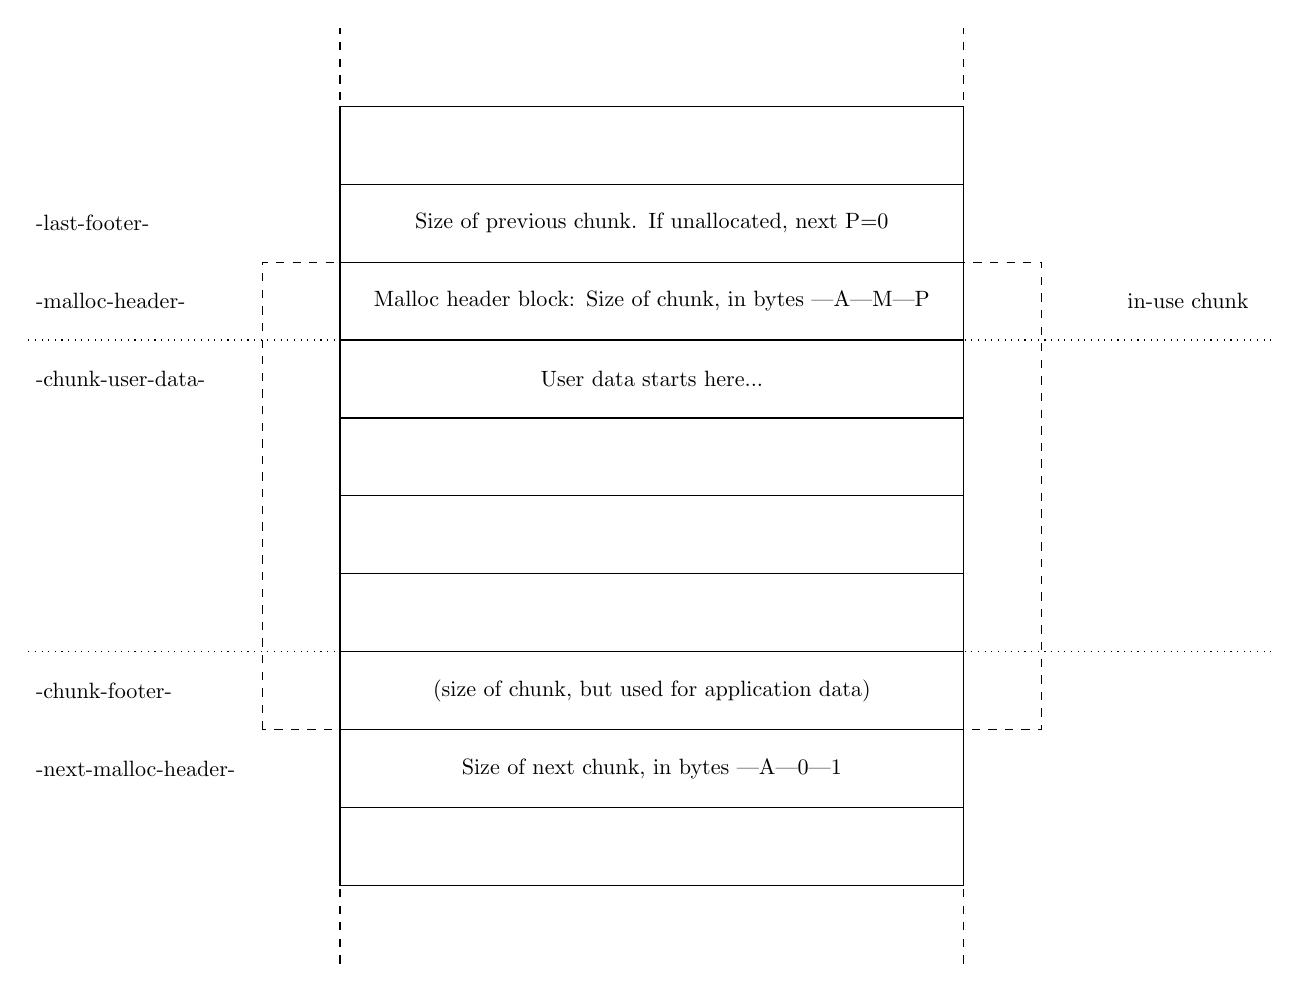
\begin{tikzpicture}[scale=0.99, every node/.style={scale=0.8}]
                % image from (0,0) to (16,12)
                
                % Draw rectangles
                \draw (4,1) rectangle (12,2);
                \draw (4,2) rectangle (12,3); % chunk-> Size of previous chunk
                \draw (4,3) rectangle (12,4); % malloc header (size of chunk)
                \draw (4,4) rectangle (12,5); %  mem-> user data starts here
                \draw (4,5) rectangle (12,6);
                \draw (4,6) rectangle (12,7);
                \draw (4,7) rectangle (12,8);
                \draw (4,8) rectangle (12,9); % nextchunk-> (app size of chunk)
                \draw (4,9) rectangle (12,10); % Size of next chunk
                \draw (4,10) rectangle (12,11);
        
                \draw[dashed] (3,3) rectangle (13,9);
                
                % after the rectangle step, the coordinates of the y axis are reversed ???
                % Dotted lines for user data
                \draw[dotted] (0,8) -- (16,8);
                \draw[dotted] (0,4) -- (16,4);
        
                % Dotted lines for memory band of 8 byte blocks
                \draw[dashed] (4,0) -- (4,12);
                \draw[dashed] (12,0) -- (12,12);
                
                % Labels
                \node[anchor=west] at (0,9.5) {-last-footer-};
                \node[anchor=west] at (0,8.5) {-malloc-header-};
                \node[anchor=west] at (0,7.5) {-chunk-user-data-};
                \node[anchor=west] at (0,3.5) {-chunk-footer-};
                \node[anchor=west] at (0,2.5) {-next-malloc-header-};
        
                \node[anchor=west] at (14,8.5) {in-use chunk};
                
                % Text inside rectangles
                \node[text width=14cm, align=center] at (8,9.5) {Size of previous chunk. If unallocated, next P=0};
                \node[text width=14cm, align=center] at (8,8.5) {Malloc header block: Size of chunk, in bytes |A|M|P};
                \node[text width=14cm, align=center] at (8,7.5) {User data starts here...};
                \node[text width=14cm, align=center] at (8,3.5) {(size of chunk, but used for application data)};
                \node[text width=14cm, align=center] at (8,2.5) {Size of next chunk, in bytes |A|0|1};
            \end{tikzpicture}
            \caption{Diagram of an allocated chunk in GLIBC 2.28 \cite{gloger_malloc_2001}.}
            \label{fig:allocated_chunk}
        \end{figure}
        
        \paragraph{}In GLIBC 2.28, the \texttt{malloc} function employs a boundary tag approach to oversee memory \glspl{chunk}. These \glspl{chunk} integrate metadata essential for memory allocation and deallocation \cite{gloger_malloc_2001} \cite{delorie_malloc_2023}. The library organizes available \glspl{chunk} into circular doubly-linked lists, termed \say{bins}, facilitating rapid retrieval of free memory \glspl{chunk} of specific sizes. However, these bins are not directly accessible in the heap dump file. To discern if a particular \gls{chunk} is occupied or available, several techniques can be employed. Primarily, the \texttt{P} bit in the malloc header serves as an indicator. A value of 1 denotes an occupied \gls{chunk}, while 0 signifies a free \gls{chunk}.

        \paragraph{}It's noteworthy that certain heap dump files appear truncated, with the concluding block being incomplete and filled with zeros. An instance of this can be observed in the final \gls{chunk} of \textit{Training/basic/V\_7\_1\_P1/24/17016-1643962152-heap.raw}.

        \begin{lstlisting}[language=bash, caption={Logs from \gls{chunk} exploration script, highlighting the last \gls{chunk} of the file \textit{Training/basic/V\_7\_1\_P1/24/17016-1643962152-heap.raw}. }]
            WARN: chunk [94022266975200] Chunk(block_index=10876, size=48176, flags=[A=False, M=False, P=True]) is out of bounds. Last block index: 16895 Iteration index: 16896 
            WARN: chunk [94022266975200] Chunk(block_index=10876, size=48176, flags=[A=False, M=False, P=True]) is out of bounds. Last block index: 16895 Iteration index: 16897
            Chunk(block_index=10876, size=48176) is only composed of zeros.
        \end{lstlisting}

        \paragraph{}A free \gls{chunk}, as per the code documentation \cite{gloger_malloc_2001}, incorporates pointers to the subsequent and preceding free \glspl{chunk} within the heap for its designated bin. The following provides a representation of a free \gls{chunk}:

        \begin{figure}[H]
            \centering
            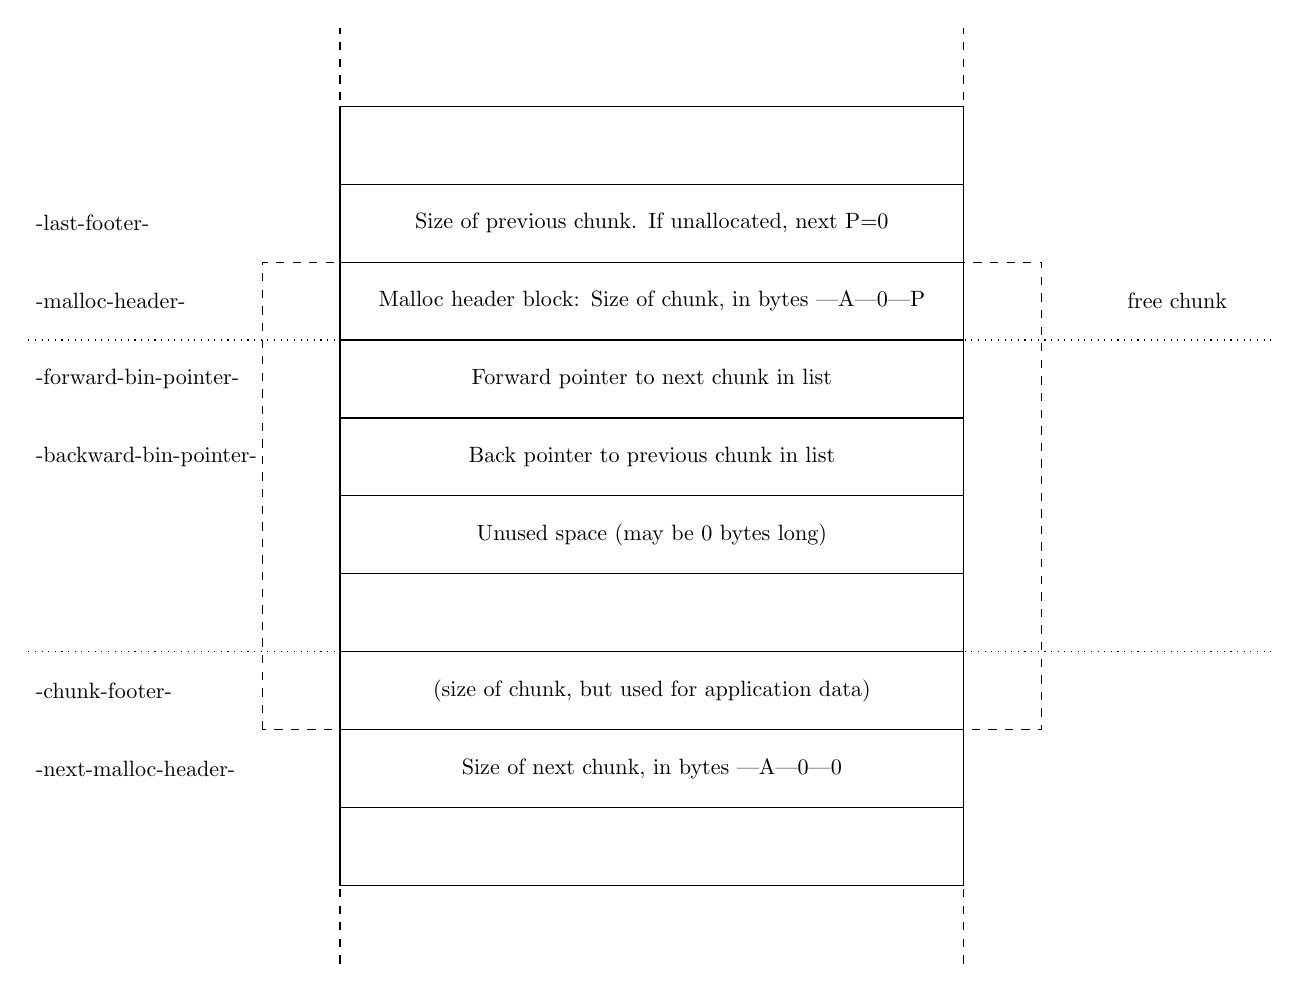
\begin{tikzpicture}[scale=0.99, every node/.style={scale=0.8}]
                % image from (0,0) to (16,12)
                
                % Draw rectangles
                \draw (4,1) rectangle (12,2);
                \draw (4,2) rectangle (12,3); % chunk-> Size of previous chunk
                \draw (4,3) rectangle (12,4); % malloc header (size of chunk)
                \draw (4,4) rectangle (12,5); %  mem-> user data starts here
                \draw (4,5) rectangle (12,6);
                \draw (4,6) rectangle (12,7);
                \draw (4,7) rectangle (12,8);
                \draw (4,8) rectangle (12,9); % nextchunk-> (app size of chunk)
                \draw (4,9) rectangle (12,10); % Size of next chunk
                \draw (4,10) rectangle (12,11);
        
                \draw[dashed] (3,3) rectangle (13,9);
                
                % after the rectangle step, the coordinates of the y axis are reversed ???
                % Dotted lines for user data
                \draw[dotted] (0,8) -- (16,8);
                \draw[dotted] (0,4) -- (16,4);
        
                % Dotted lines for memory band of 8 byte blocks
                \draw[dashed] (4,0) -- (4,12);
                \draw[dashed] (12,0) -- (12,12);
                
                % Labels
                \node[anchor=west] at (0,9.5) {-last-footer-};
                \node[anchor=west] at (0,8.5) {-malloc-header-};
                \node[anchor=west] at (0,3.5) {-chunk-footer-};
                \node[anchor=west] at (0,2.5) {-next-malloc-header-};
    
                \node[anchor=west] at (0,7.5) {-forward-bin-pointer-};
                \node[anchor=west] at (0,6.5) {-backward-bin-pointer-};
        
                \node[anchor=west] at (14,8.5) {free chunk};
                
                % Text inside rectangles
                \node[text width=14cm, align=center] at (8,9.5) {Size of previous chunk. If unallocated, next P=0};
                \node[text width=14cm, align=center] at (8,8.5) {Malloc header block: Size of chunk, in bytes |A|0|P};
                \node[text width=14cm, align=center] at (8,7.5) {Forward pointer to next chunk in list};
                \node[text width=14cm, align=center] at (8,6.5) {Back pointer to previous chunk in list};
                \node[text width=14cm, align=center] at (8,5.5) {Unused space (may be 0 bytes long)};
                \node[text width=14cm, align=center] at (8,3.5) {(size of chunk, but used for application data)};
                \node[text width=14cm, align=center] at (8,2.5) {Size of next chunk, in bytes |A|0|0};
            \end{tikzpicture}
            \caption{Diagram of a free chunk in GLIBC 2.28 \cite{gloger_malloc_2001}.}
            \label{fig:free_chunk}
        \end{figure}

        \paragraph{}The principle of \textbf{chunk chaining}\label{seq:background:chunk_chaining} is pivotal for navigating the heap dump file. By adhering to the sequence of malloc headers, we can systematically traverse the allocated memory chunks within the heap dump. This methodology is corroborated by the source code, which contains a comment indicating that, given the address of the initial chunk (the one with the lowest address) in a heap, one can iterate over all the chunks by leveraging the size data.

        \paragraph{}Throughout the development of scripts and tools for this thesis, we've integrated various checks and validations to ensure the consistency of this chunk chaining assumption. Should any discrepancies arise, the tools are designed to flag an error, and typically bypass the problematic data. Such a design choice aims to fortify the tools against unforeseen data structures and to bolster the reliability of the outcomes.

